\section{Анализ предметной области}

В этом разделе будут проведен анализ предметной области: даны понятия ядра Linux, страниц памяти и механизма виртуальной памяти.

\subsection{Ядро Linux}

Ядро Linux \cite{linux} -- ядро операционной системы с открытым исходным кодом, распространяющееся как свободное программное обеспечение. Ядро Linux является монолитным, то есть содержит в себе все функции, возлагаемые на операционную систему и работает в одном адресном пространстве. При разработке ядра из микроядерной модели были позаимствованы некоторые решения: модульный принцип построения, приоритетное планирование самого себя, поддержка многопоточного режима и динамической загрузки в ядро внешних бинарных файлов (модулей ядра) \cite{kernel-development}. 

Ниже представлены отличительные черты ядра Linux:

\begin{itemize}
	\item потоки ничем не отличаются от обычных процессов. С точки зрения ядра все процессы одинаковы и лишь некоторые из них делят ресурсы между собой;
	\item динамическая загрузка модулей ядра;
	\item приоритетное планирование. Ядро способно прервать выполнение текущего процесса, даже если оно выполняется в режиме ядра;
	\item объектно-ориентированная модель устройств. Ядро поддерживает классы устройств и события;
	\item ядро Linux является результатом свободной и открытой модели разработки \cite{kernel-development}.
\end{itemize}

\subsection{Страницы памяти}

Работа с памятью в ядре Linux организована с помощью примитива страниц. Страница памяти -- набор из $n$ байт, непрерывно расположенных в памяти. Наименьшими адресуемыми единицами памяти в системе являются байт и машинное слово, но такой подход не является удобным \cite{kernel-development}. Размер страницы это аппаратно зависимая, фиксированная константа \texttt{PAGE\_SIZE}, объявленная в исходном коде ядра Linux. На большинстве современных архитектур, поддерживаемых Linux, размер страницы составляет 4 Кб \cite{4kb-page-size}. Страничная организация памяти позволяет реализовать механизм виртуальной памяти.

В ядре Linux каждая физическая страница памяти описывается с помощью структуры \texttt{struct page}, которая имеет большое количество полей, часть из которых используется по разному, в зависимости от текущей ситуации. 

\subsection{Виртуальная память}

Виртуальная память -- специальный механизм организации памяти, при котором процессы работают не с физическими адресами напрямую, а с линейными. Трансляция линейных адресов в физические чаще всего реализована аппаратно, с помощью блока управления памяти (англ. memory managment unit -- MMU \cite{mmu}). Кроме того, существует аппаратный способ ускорения трансляции -- буффер ассоциативной трансляции (англ. translation lookaside buffer -- TLB \cite{tlb}). В связи с этим, можно сделать вывод о относительной быстроте трансляции адресов, что никак не сказывается на отзывчивости системы.

Механизм виртуальной памяти обладает следующими преимуществами:

\begin{itemize}
	\item изоляция пользовательских процессов друг от друга;
	\item возможность использовать больше оперативной памяти, чем её физически установлено в системе;
	\item нет необходимости управлять общим адресным пространством.
\end{itemize}

Ядро Linux поддерживает механизм виртуальной памяти и реализовывает его с помощью таблиц страниц. Данная структура данных позволяет из линейного адреса ячейки памяти получить физический. Схема работы таблиц страниц представлена на рисунке \ref{fig:tables}.

\begin{figure}[h]
	\centering
	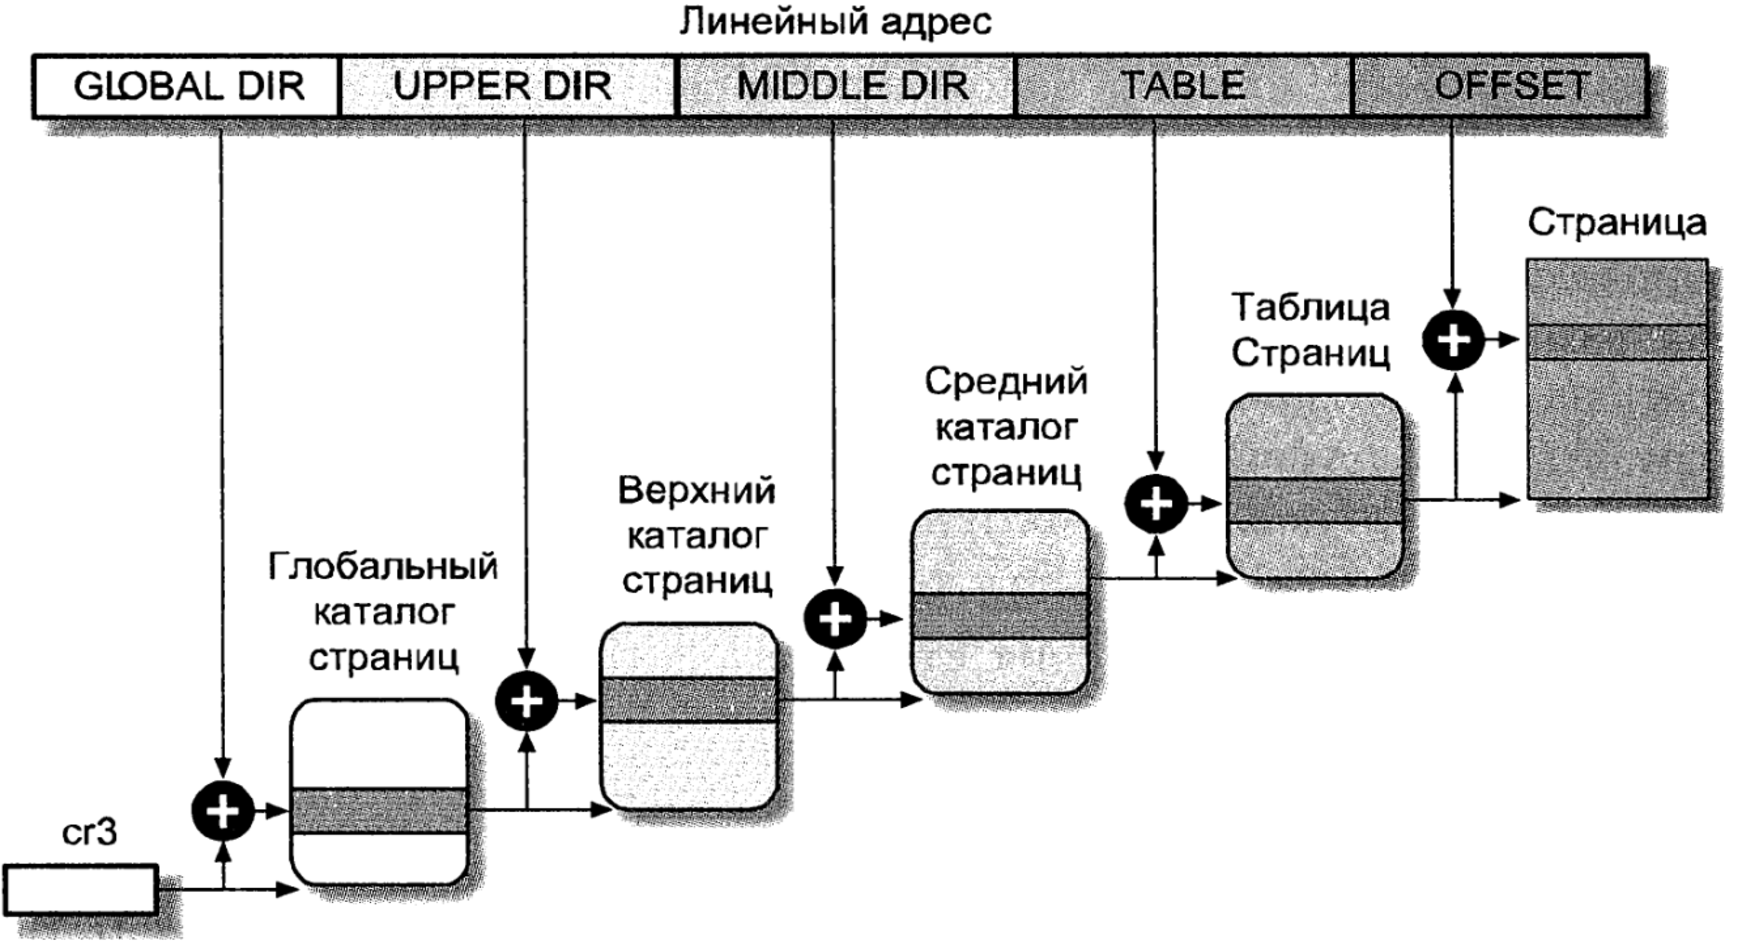
\includegraphics[width=\textwidth]{img/tables.png}
	\caption{Трансляция линейного адреса в физический}
	\label{fig:tables}
\end{figure}

Для преобразования линейного адреса в физический, ядро Linux использует 3 каталога и таблицу страниц:

\begin{itemize}
	\item глобальный каталог страниц;
	\item верхний каталог страниц;
	\item средний каталог страниц;
	\item таблица страниц;
\end{itemize}

Элементами этих каталогов являются адреса, указывающие на начало соответствующего каталога. Глобальный каталог указывает на верхний каталог, верхний на средний, средний на таблицу страниц, а таблица страница на физический адрес искомой страницы. В самом линейном адресе находятся смещения от начала соответствующего каталога. Адрес глобального каталога страниц обычно хранится в некотором регистре -- например, на архитектуре х86, этот регистр называется CR3. Каждый процесс в системе имеет свою собственную таблицу страниц.

\section{Существующие методы распределения памяти}

В данном разделе будут рассмотрены методы распределения памяти, представленные в ядре Linux. Рассмотренные методы распределения памяти будут классифицированы, сделаны вывод о подходящей сфере задач, в которых рассмотренные методы будут наиболее эффективны.

\subsection{Алгоритм <<Buddy-система>>}

При частом выделении групп смежных страниц физической памяти ядро должно придерживаться устойчивой и эффективной стратегии. Наиболее известная проблема, с которой сталкивается ядро решая данную задачу, называется внешней фрагментацией. Суть заключается в том, что частые запросы на выделение и освобождение смежных групп страниц разного размера приводит к ситуации, когда несколько небольших участков памяти свободных страниц находятся внутри выделенных страниц. Это может привести к тому, что в системе есть запрашиваемое количество свободных страниц, но она всё равно не может удовлетворить запрос. 

Существует два метода борьбы с внешней фрагментацией:

\begin{itemize}
	\item аппаратный -- использование электронной схемы, позволяющей отображать группы несмежных свободных страниц в непрерывные интервалы линейных адресов;
	\item программный -- использовать алгоритм, позволяющий избегать разбиения большого свободного блока страниц ради удовлетворения запроса на меньший блок.
\end{itemize}

Ядро Linux решает проблему внешней фрагментации с помощью алгоритма buddy-системы. Все свободные страниц памяти объединяются в 11 списков, содержащие блоки состоящие из $2^k$ смежных страниц, где $k = 0..10$. Физический адрес самого первого страничного кадра в блоке кратен размеру группы: $address \ mod \ k = 0$. Таким образом, количество запрашиваемых страниц у аллокатора, использующего алгоритм buddy-систем, должно быть кратно степеням двойки.

При запросе группы, состоящей из $2^k$ смежных страниц памяти, алгоритм проверяет наличие свободного блока в списке блоков, которые содержат $2^k$ смежных страниц памяти. Если блок найден, алгоритм возвращает адрес первой смежной страницы памяти из найденного блока, удаляет блок из свободного списка и завершает свою работу. В обратном случае (если такой блок не найден), алгоритм продолжает поиск свободного блока в списке из $2^(k + 1)$ смежных страниц памяти. В случае успеха, алгоритм переносит блок из $2^k$ страниц в соответствующий ему список, а оставшиеся $2^k$ страниц выделяет для удовлетворения запроса. Если блок не найден, алгоритм продолжает поиск в списке из $2^(k + 2)$ смежных страниц, в случае успеха итеративно перенося часть страниц в соответствующие списки блоков. Если не в одном из списков не было найдено ни одного свободного блока, алгоритм завершается и сигнализирует об ошибке. 

При освобождении блоков страниц, ядро пытается слить пары buddy-блоков размера $S$ в один блок размера $2S$ (отсюда и взялось название buddy (приятель)). Два блока считаются buddy-блоками, если:

\begin{itemize}
	\item оба блока имеют одинаковый размер $S$;
	\item они являются смежными физическими;
	\item выполняется условие $address\ mod\ (2 * S) = 0$, где $address$ -- физический адрес первой страницы в первом блоке.
\end{itemize}

Ниже приведем пример работы алгоритма при запросе $2^0 = 1$ страниц (cм. рисунки \ref{fig:buddy-alloc-1} - \ref{fig:buddy-alloc-4})

\begin{figure}[h]
	\centering
	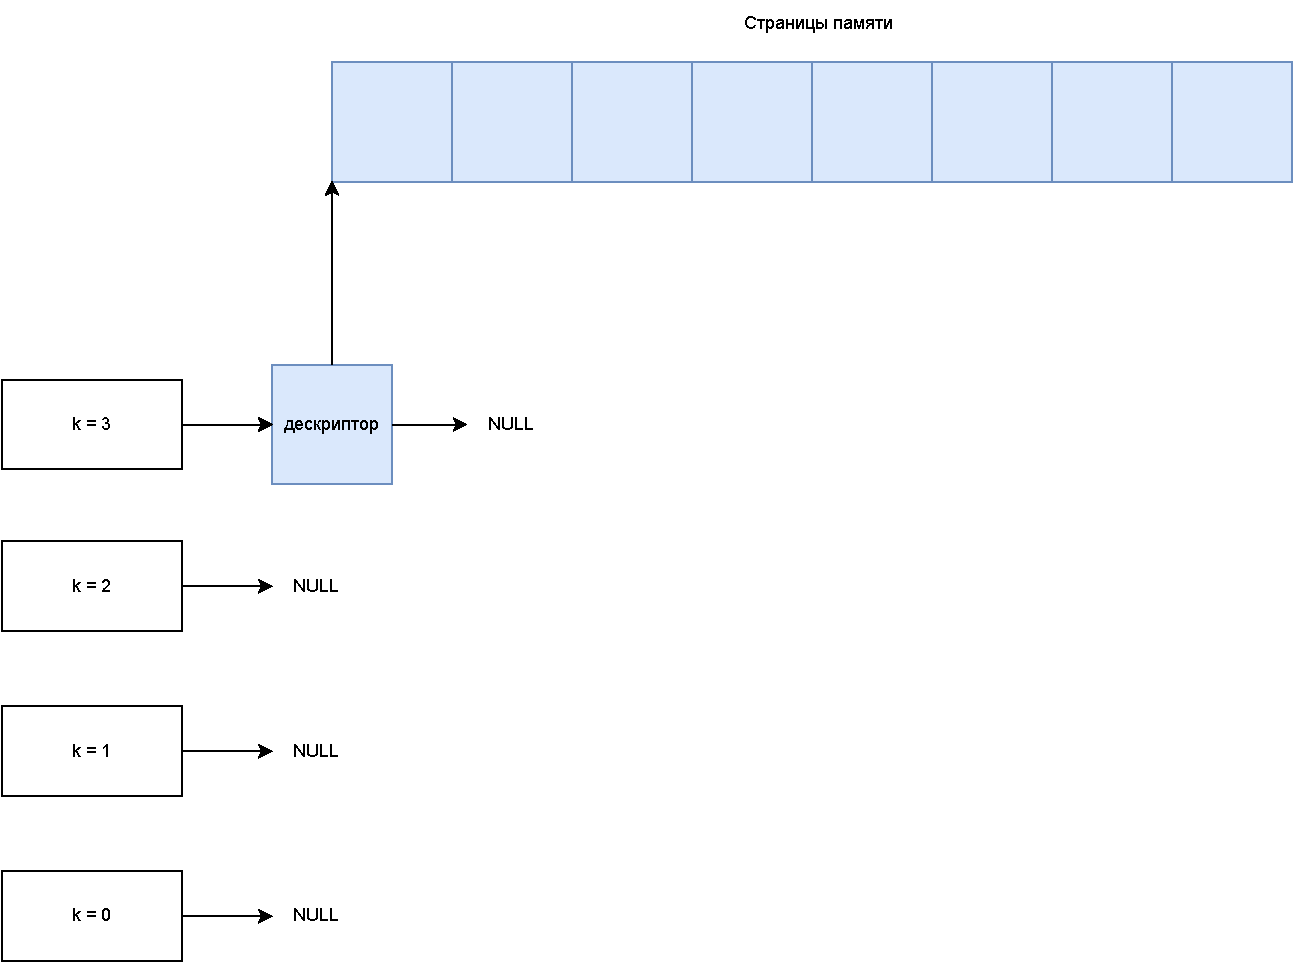
\includegraphics[width=\textwidth]{img/buddy-allocator-1.pdf}
	\caption{Пример работы алгоритма buddy-системы, часть 1}
	\label{fig:buddy-alloc-1}
\end{figure}

1. Алгоритм обошёл все списки свободных блоков начиная с $k = 0$, найдя свободный блок в списке с $k = 3$. В данном списке оказался один свободный блок, отмеченный голубым цветом (см. рис \ref{fig:buddy-alloc-1}).

\begin{figure}[h]
	\centering
	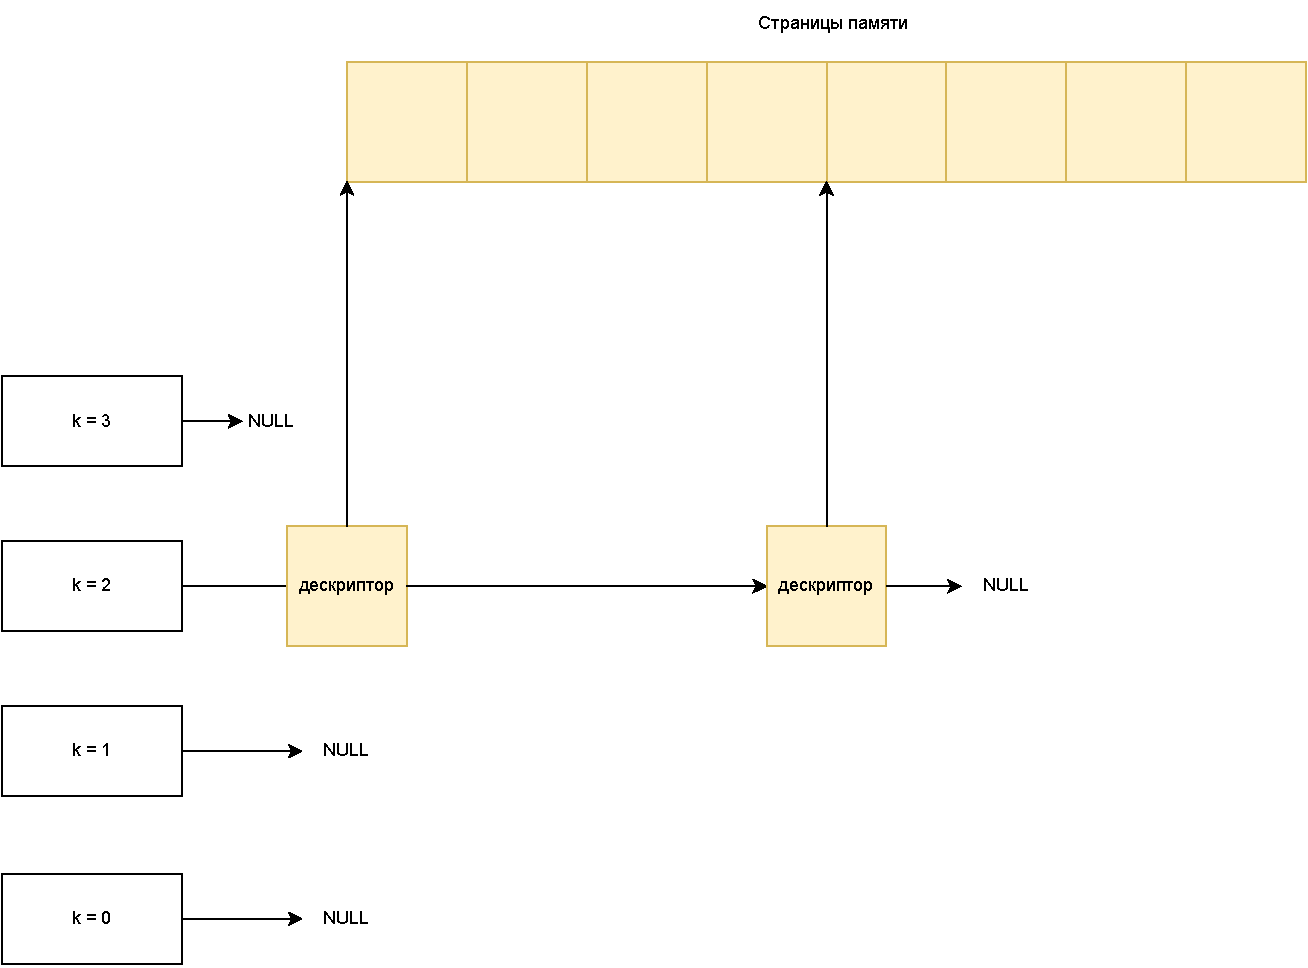
\includegraphics[width=\textwidth]{img/buddy-allocator-2.pdf}
	\caption{Пример работы алгоритма buddy-системы, часть 2}
	\label{fig:buddy-alloc-2}
\end{figure}

2. Далее, алгоритм разбивает блок из списка с $k = 3$ на два блока с $k = 2$, добавляя их в соответствующий список. Блоки с $k = 2$ на рисунке \ref{fig:buddy-alloc-2} отмечены жёлтым цветом. 

\begin{figure}[h]
	\centering
	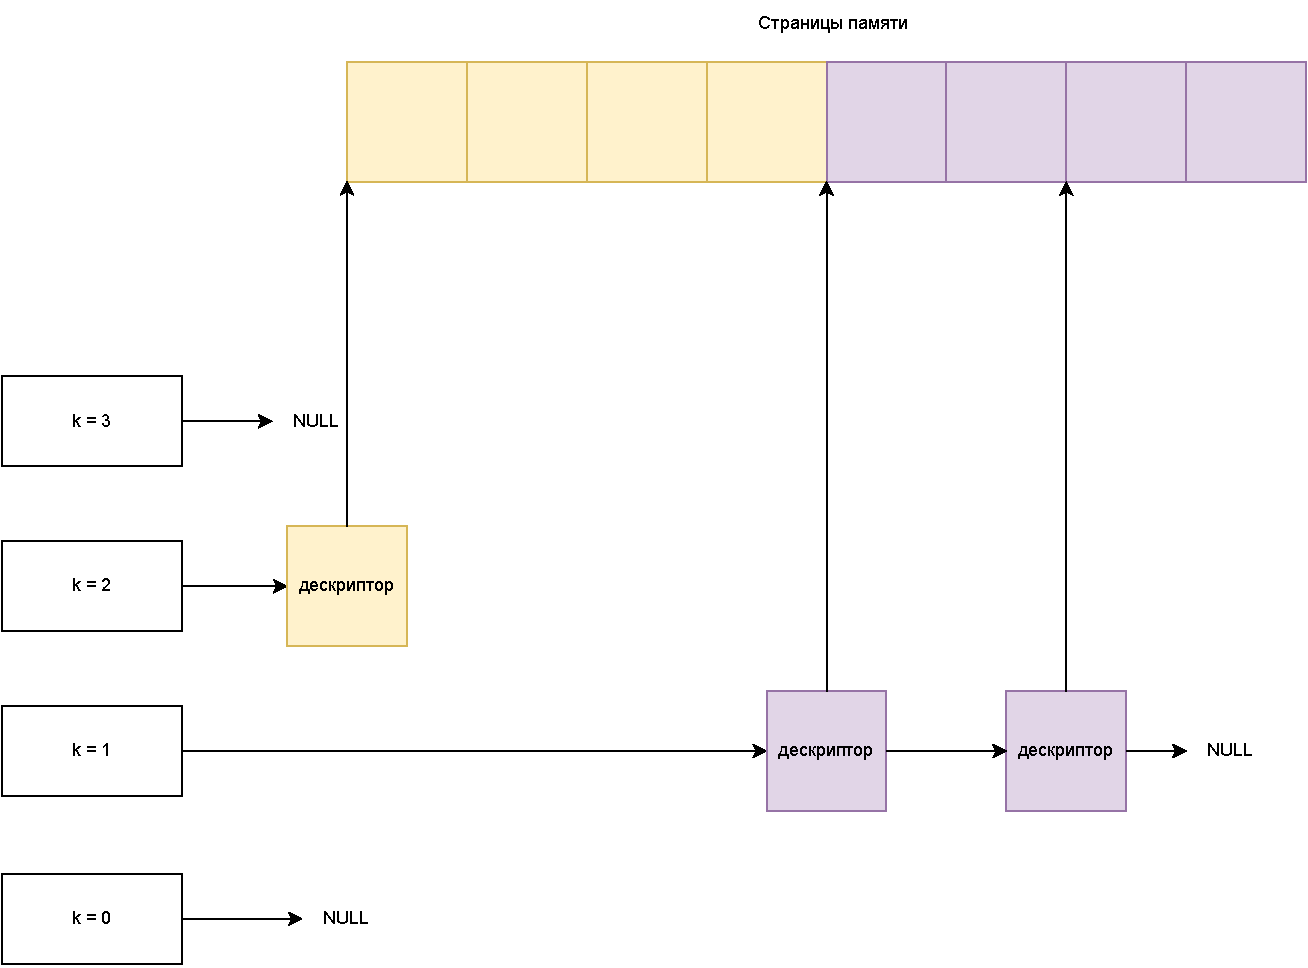
\includegraphics[width=\textwidth]{img/buddy-allocator-3.pdf}
	\caption{Пример работы алгоритма buddy-системы, часть 3}
	\label{fig:buddy-alloc-3}
\end{figure}

3. Разбиение продолжается: один из блоков из списка с $k = 2$ разбивается на два блока с $k = 1$, которые отмечены на рисунке \ref{fig:buddy-alloc-1} фиолетовым цветом.

\begin{figure}[h]
	\centering
	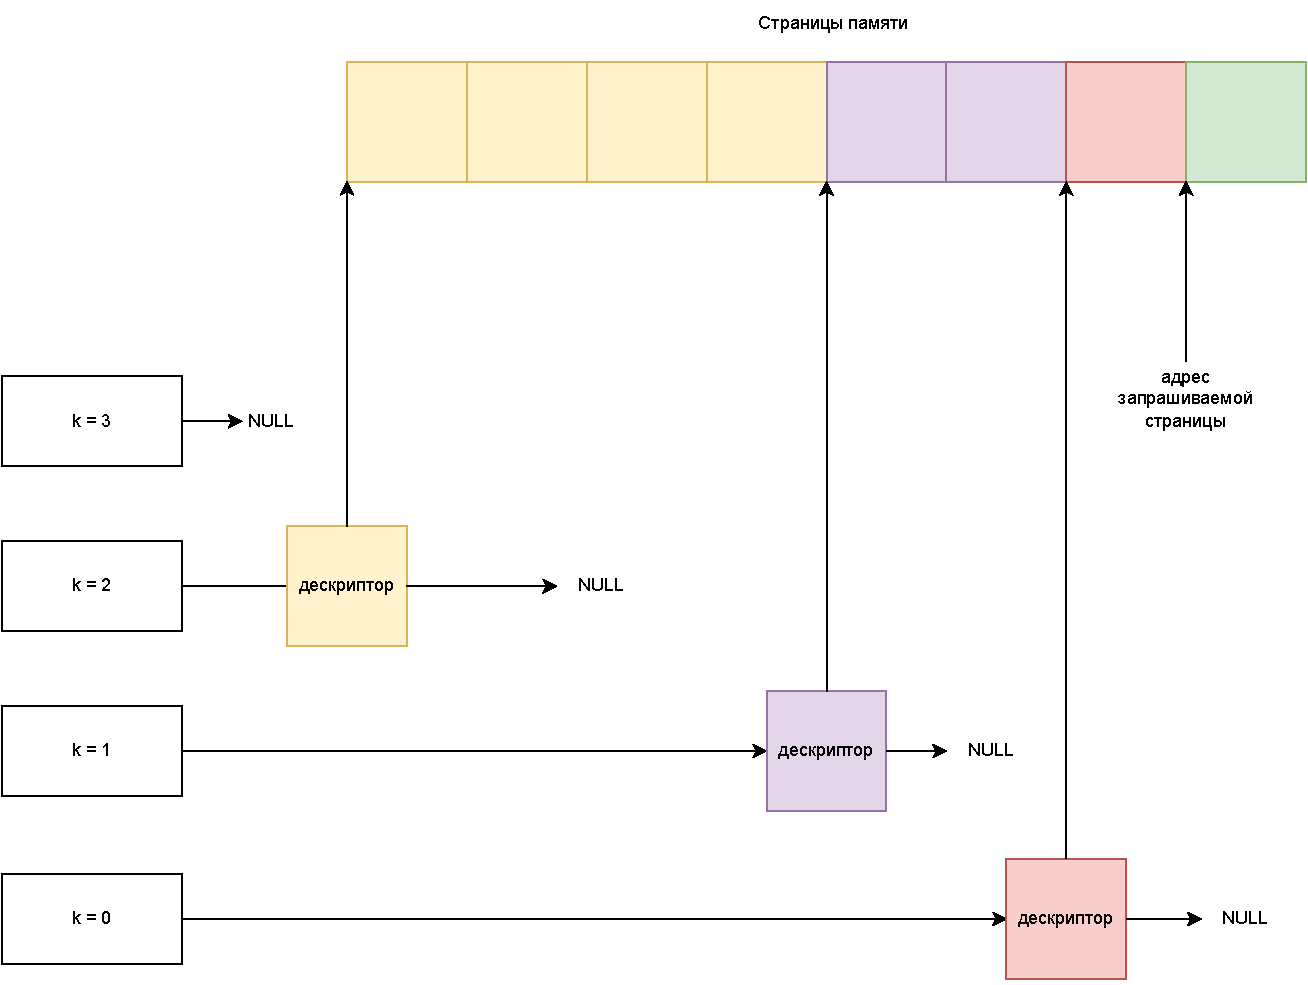
\includegraphics[width=\textwidth]{img/buddy-allocator-4.pdf}
	\caption{Пример работы алгоритма buddy-системы, часть 4}
	\label{fig:buddy-alloc-4}
\end{figure}

4. Наконец, разбив один из блоков из списка с $k = 1$ на два блока с $k = 0$, помеченные красным цветом на рисунке \ref{fig:buddy-alloc-4}, алгоритм находит подходящую смежную область, отмеченную зеленым цветом, (в данном примере это одна страница, т.к. $k = 0$) и завершает свою работу.

При попытке освобождения блока работа алгоритма аналогична, но выполняется наооборот. В конечном итоге, при освобождении ранее запрошенного у системы зеленого блока (см. рисунок \ref{fig:buddy-alloc-4}), в системе останется один свободный блок с $k = 3$ (см. рисунок \ref{fig:buddy-alloc-1}).

\subsubsection{Реализация в ядре Linux}

Реализация в ядре Linux построена на двух структурах данных:

\begin{itemize}
	\item \texttt{mem\_map} -- глобальная переменная, массив типа \texttt{struct page}, описывающая всю физическую память в системе. Первый элемент массива описывает первую физической странице памяти, второй - вторую, и так далее.
	\item массив структур типа \texttt{struct free\_area}.
\end{itemize}

Массив, состоящий из 11 элементов и указывающий на списки блоков (дескрипторы свободных смежных областей памяти), описывается с помощью массива структур типа \texttt{struct free\_area}. Объявление данной структуры представлено в листинге \ref{code:free_area}.

\begin{code}
	\captionof{listing}{Структура \texttt{struct free\_area}}
	\label{code:free_area}
	\inputminted
	[
	frame=single,
	framerule=0.5pt,
	framesep=20pt,
	fontsize=\small,
	tabsize=4,
	linenos,
	numbersep=5pt,
	xleftmargin=10pt,
	]
	{text}
	{code/free_area.c}
\end{code}

Структура содержит внутри себя два поля:

\begin{itemize}
	\item \texttt{free\_list} -- список всех блоков (дескрипторов), в том числе занятых, указывающие на соответствующие им смежные участки памяти из $2^k$ свободных страниц;
	\item \texttt{nr\_free} -- количество свободных блоков в списке.
\end{itemize}

Выделение блоков возможно с помощью функции \texttt{alloc\_pages}, а освобождение используя \texttt{free\_pages}. Сигнатуры этих функций представлены в листингах \ref{code:alloc_pages} - \ref{code:free_pages}.

\begin{code}
	\captionof{listing}{Сигнатура функции \texttt{alloc\_pages}}
	\label{code:alloc_pages}
	\inputminted
	[
	frame=single,
	framerule=0.5pt,
	framesep=20pt,
	fontsize=\small,
	tabsize=4,
	linenos,
	numbersep=5pt,
	xleftmargin=10pt,
	]
	{text}
	{code/alloc_pages.c}
\end{code}

Функция \texttt{alloc\_pages} принимает два параметра:

\begin{itemize}
	\item \texttt{gfp} -- набор флагов, используемых при аллокации. Например, при указании флага \texttt{GFP\_ATOMIC}, что запрос на выделения памяти должен пройти атомарно, что означает что вызывающий тракт ядра не может быть блокирован, либо завершиться неудачей.
	\item \texttt{order} -- порядок запрашиваемого смежного блока страниц, т.е. $S = 2^k$, где $S$ -- количество физических смежных страниц памяти.
\end{itemize}

Функция возвращает указатель на дескриптор типа \texttt{struct page} первой страницы из запрашиваемого участка смежных страниц.

\begin{code}
	\captionof{listing}{Сигнатура функции \texttt{free\_pages}}
	\label{code:free_pages}
	\inputminted
	[
	frame=single,
	framerule=0.5pt,
	framesep=20pt,
	fontsize=\small,
	tabsize=4,
	linenos,
	numbersep=5pt,
	xleftmargin=10pt,
	]
	{text}
	{code/free_pages.c}
\end{code}

Функция \texttt{free\_pages} так же принимает два параметра:

\begin{itemize}
	\item \texttt{addr} -- физический адрес первой страницы освобождаемого блока смежных страниц;
	\item \texttt{order} -- порядок освобождаемого блока.
\end{itemize}

Реализация алгоритма выделения и освобождения смежных блоков страниц памяти в ядре Linux аналогична алгоритму описанному в прошлой главе. Алгоритм работает с физически смежными страница памяти, например, при $order = 3$, алгоритм выделит блок из $2^3 = 8$ физически смежных страниц оперативной памяти. Рассматриваемый метод работает со страницами памяти, то есть минимум он сможет выделить \texttt{PAGE\_SIZE} (обычно 4096) байт. При необходимости использовать менее чем \texttt{PAGE\_SIZE} байт, часть памяти будет не использована вовсе. Использовать страницу целиком, для хранения нескольких байтов -- расточительно.

\subsection{Управление областями памяти}

Область памяти -- последовательность ячеек, имеющих смежные физические адреса и произвольную длину. Buddy-аллокации не подходит для выделения таких областей памяти, потому что работает со страницами, размер которых статичен. 

В ядре Linux принят следующий подход к управлению такими областями: размер областей привязан к степеням двойки, размеры расположены в диапазоне от 32 до 131 072 (геометрическая прогрессия). Такой подход позволяет бороться с внутренней фрагментацией (несоответствие между размером запрашиваемой памяти к выделенной для удовлетворения запроса) и гарантирует что она всегда будет меньше 50\%. То есть, при запросе $k$ байт, число $k$ будет округлено до ближайшей (в большую сторону) степени двойки.

\subsubsection{Slab аллокатор}

Функции ядра многократно запрашивают области памяти одного и того же размера, например, под дескрипторы (структуры) описывающие что-либо. Когда ядро создаёт новый процесс, оно выделяет области памяти под несколько структур фиксированного размера: дескриптор процесса, дескриптор файла и так далее. 

Запросы на участки памяти фиксированного размера, про которые известно, что они возникают часто, можно эффективно обрабатывать создав пулл из объектов имеющих соответствующий размер. Такой способ помогает избежать внутренней фрагментации. Редкие запросы на участки памяти, можно обрабатывать с использованием схемы, основанной на применении объектов с геометрически распределенными размерами, как было описано ранее.

Slab аллокатор группирует объекты в кэши, каждый кэш предназначен для выделение объектов одного типа, и, соответственно, одного и того же размера. Например, для выделения участка памяти, в котором будет располагаться структура \texttt{struct file}, будет использован один кэш, а для структуры \texttt{struct task\_struct} будет использован другой кэш.

В ядре Linux каждый slab кэш описывается с помощью структуры \texttt{struct kmem\_cache}, описание которой, с наиболее важными полями, представлено в листинге \ref{code:kmem_cache}.

\begin{code}
	\captionof{listing}{Структура \texttt{struct kmem\_cache}}
	\label{code:kmem_cache}
	\inputminted
	[
	frame=single,
	framerule=0.5pt,
	framesep=20pt,
	fontsize=\small,
	tabsize=4,
	linenos,
	numbersep=5pt,
	xleftmargin=10pt,
	]
	{text}
	{code/kmem_cache.c}
\end{code}

Подробное описание полей структуры \texttt{struct kmem\_cache}:

\begin{itemize}
	\item \texttt{size} -- общий размер кэша;
	\item \texttt{flags} -- флаги, используемые при аллокации;
	\item \texttt{num} -- количество объектов, хранящихся в кэше;
	\item \texttt{name} -- строка, имя кэша;
	\item \texttt{list} -- циклический двунаправленный список всех кэшей в системе;
	\item \texttt{refcount} -- количество ссылок на кэш в системе. В случае, если \texttt{refcount} = 0, система удалит кэш.
	\item \texttt{object\_size} -- размер объектов, хранящихся в кэше;
	\item \texttt{align} -- выравнивание объектов в памяти;
	\item \texttt{node} -- массив структур типа \texttt{struct kmem\_cache\_node} (см. листинг \ref{code:kmem_cache_node})
\end{itemize}

Таким образом, структура \texttt{struct kmem\_cache} описывает кэш в целом, и хранит указатель на структуру \texttt{struct kmem\_cache\_node}, описанную в листинге \ref{code:kmem_cache_node}.

\begin{code}
	\captionof{listing}{Структура \texttt{struct kmem\_cache\_node}}
	\label{code:kmem_cache_node}
	\inputminted
	[
	frame=single,
	framerule=0.5pt,
	framesep=20pt,
	fontsize=\small,
	tabsize=4,
	linenos,
	numbersep=5pt,
	xleftmargin=10pt,
	]
	{text}
	{code/kmem_cache_node.c}
\end{code}

Структура \texttt{struct kmem\_cache\_node} хранит указатели на списки трех типов:

\begin{itemize}
	\item \texttt{slabs\_partial} -- в этом списке хранятся дескрипторы участков памяти как со свободными, так и с несвободными объектами;
	\item \texttt{slabs\_full} -- дескрипторы полностью заполненных участков памяти;
	\item \texttt{slabs\_free} -- дескрипторы полностью свободных участков памяти.
\end{itemize}

В рассматриваемой структуре так же хранятся дополнительные поля, упрощающие работу с вышеописанными списками:

\begin{itemize}
	\item \texttt{total\_slabs} -- количество все дескрипторов;
	\item \texttt{free\_slabs} -- количество свободных дескрипторов;
	\item \texttt{free\_objects} -- общее количество всех свободных объектов.
\end{itemize}

Каждый участок памяти в кэше имеет собственный дескриптор типа \texttt{struct slab}, описание которого приводится в листинге \ref{code:slab}.

\begin{code}
	\captionof{listing}{Структура \texttt{struct slab}}
	\label{code:slab}
	\inputminted
	[
	frame=single,
	framerule=0.5pt,
	framesep=20pt,
	fontsize=\small,
	tabsize=4,
	linenos,
	numbersep=5pt,
	xleftmargin=10pt,
	]
	{text}
	{code/slab.c}
\end{code}

Данная структура содержит в себе несколько полей:

\begin{itemize}
	\item \texttt{slab\_list} -- указатели, используемые в одном из трех двунаправленных списокв дескрипторов участков памяти (см. листинг \ref{kmem_cache_node});
	\item \texttt{slab\_cache} -- указатель на структуру типа \texttt{struct kmem\_cache}, описанную в листинге \ref{code:kmem_cache};
	\item \texttt{freelist} -- массив индексов всех свободных объектов;
	\item \texttt{s\_mem} -- адрес первого объекта в участке;
	\item \texttt{inuse} -- количество несвободных объектов в участке памяти;
\end{itemize}

Взаимосвязи между структурами, которые были описаны выше, представлены на рисунке \ref{fig:kmem_cache}. Красным цветом отмечены занятые объекты, зеленным -- свободные.

\begin{figure}[h]
	\centering
	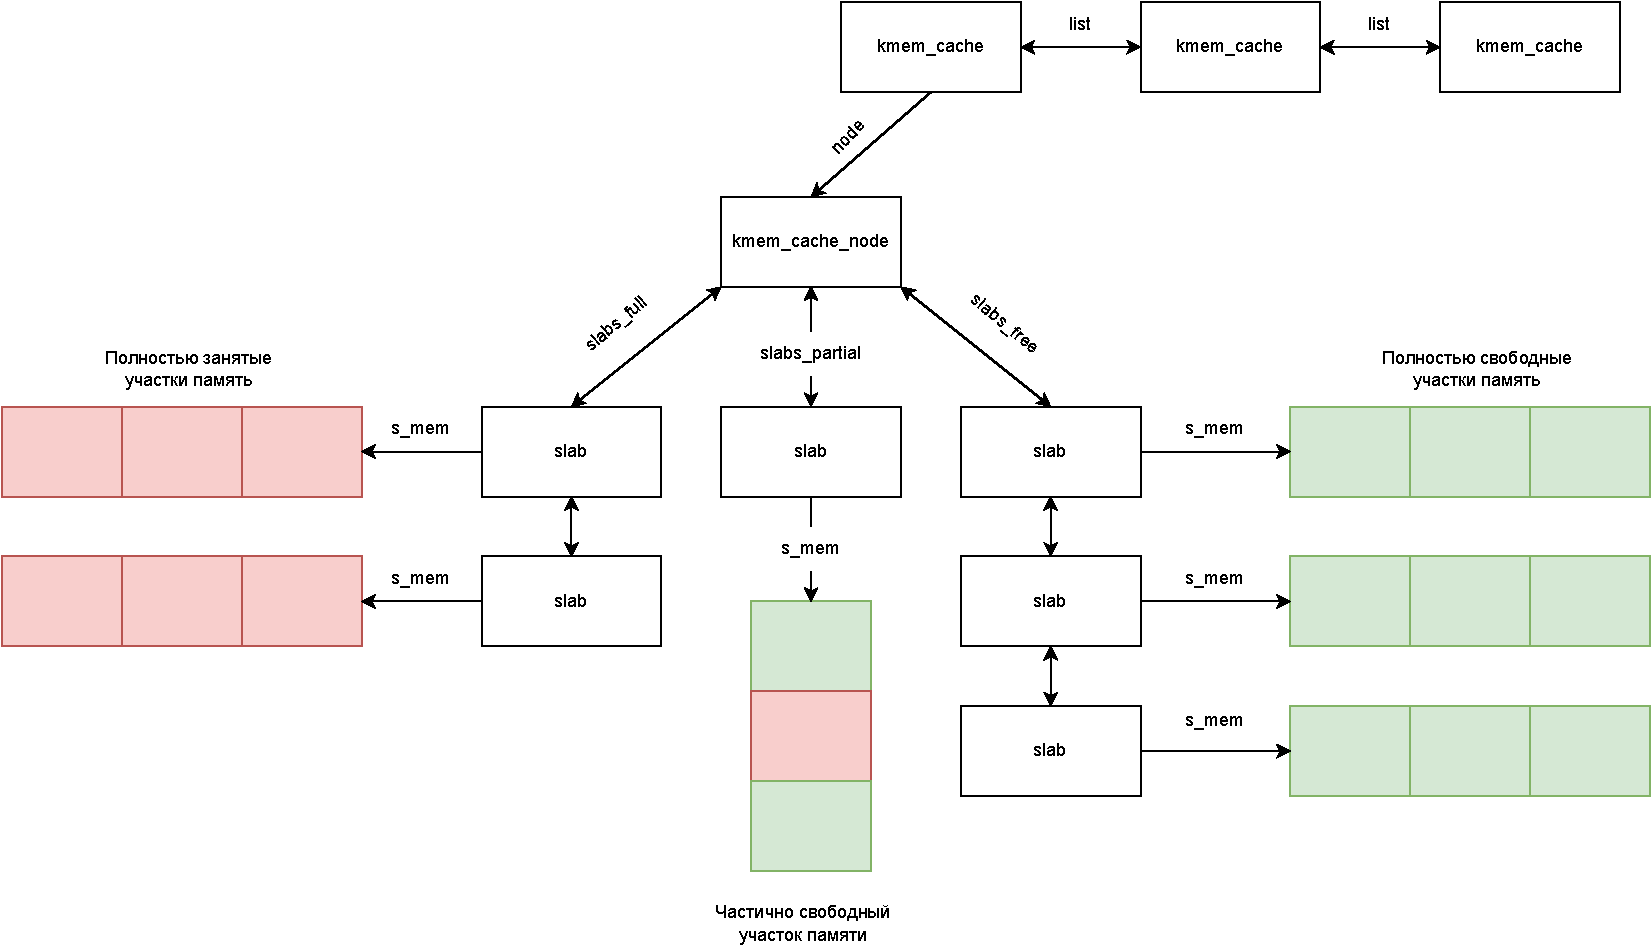
\includegraphics[width=\textwidth]{img/kmem_cache.pdf}
	\caption{Взаимосвязи между структурами данных, используемые в работе Slab аллокатора.}
	\label{fig:kmem_cache}
\end{figure}

На рисунке \ref{fig:cache_objects} показана взаимосвязь между дескрипторами участков (\texttt{struct slab}) и объектами в памяти. Красным цветом отмечены занятые объекты, зеленным -- свободные.

\begin{figure}[h]
	\centering
	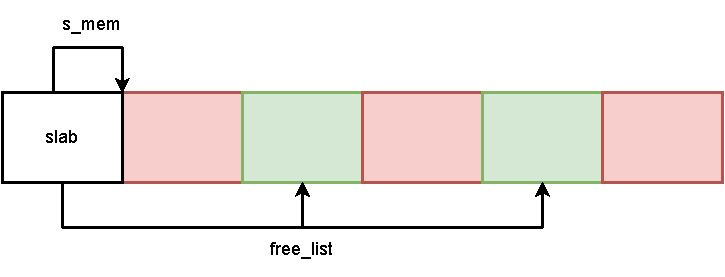
\includegraphics[width=\textwidth]{img/kmem_cache_2.pdf}
	\caption{Описание работы структуры \texttt{struct slab}.}
	\label{fig:cache_objects}
\end{figure}

Для работы со slab аллокатором в ядре Linux используется API, представленное в листинге \ref{code:slab_cache_api}


\begin{code}
	\captionof{listing}{API для работы с Slab кэшем в ядре Linux}
	\label{code:slab_cache_api}
	\inputminted
	[
	frame=single,
	framerule=0.5pt,
	framesep=20pt,
	fontsize=\small,
	tabsize=4,
	linenos,
	numbersep=5pt,
	xleftmargin=10pt,
	]
	{text}
	{code/kmem_cache_api.c}
\end{code}

\begin{itemize}
	\item \texttt{kmem\_cache\_create} -- создать Slab кэш с именем \texttt{name} размером \texttt{size}. Возвращает указатель на структуру типа \texttt{struct kmem\_cache}.
	\item \texttt{kmem\_cache\_alloc} -- запросить объект в Slab кэше \texttt{s};
	\item \texttt{kmem\_cache\_free} -- освободить объект \texttt{objp} в кэше \texttt{s};
	\item \texttt{kmem\_cache\_destroy} -- уничтожить кэш \texttt{s};
\end{itemize}

Функции, описанные выше, используются для создания кэша, который хранит объекты определенного размера. В случае, если системе требуются участки памяти разной длинны, и такие запросы редки, следует использовать пару функции \texttt{kmalloc} и  \texttt{kfree}, сигнатуры которых представлены в листинге \ref{code:kmalloc-kfree}. 

\begin{code}
	\captionof{listing}{Сигнатуры функций \texttt{kmalloc} и \texttt{kfree}}
	\label{code:kmalloc-kfree}
	\inputminted
	[
	frame=single,
	framerule=0.5pt,
	framesep=20pt,
	fontsize=\small,
	tabsize=4,
	linenos,
	numbersep=5pt,
	xleftmargin=10pt,
	]
	{text}
	{code/kmalloc-kfree.c}
\end{code}

Функция \texttt{kmalloc} так же использует Slab аллокатор, обрабатывая запрос с помощью группы общих кэшей размером от 32 до 131 072 байт. Таким образом, размер области памяти, запрашиваемый у системы округляется к ближайшей степени двойки.

\subsubsection{Пулы памяти}

Пул памяти -- резерв динамической области памяти, выделенной для конкретного компонента ядра, то есть использовать память может только тот компонент, который этот пул создал. Обычно, такой пул памяти создается в помощь slab аллокатору, т.е. используется в качестве резерва объектов для участков памяти. В ядре Linux такой пул описывается с помощью структуры \texttt{struct mempool\_t}, поля которой представлены в листинге \ref{code:mempool_t}.

\begin{itemize}
	\item \texttt{min\_nr} -- максимальное количество элементов в пуле;
	\item \texttt{curr\_nr} -- текущее количество элементов в пуле;
	\item \texttt{elements} -- указатель на массив указателей на зарезервированные элементы;
	\item \texttt{pool\_data} -- специальные данные, используемые владельцем пула;
	\item \texttt{alloc} -- метод для выделения памяти;
	\item \texttt{free} -- метод для освобождения элемента;
	\item \texttt{wait} -- очередь, используемая, когда пул памяти пуст.
\end{itemize}

\pagebreak

\begin{code}
	\captionof{listing}{Структура \texttt{mempool\_t}}
	\label{code:mempool_t}
	\inputminted
	[
	frame=single,
	framerule=0.5pt,
	framesep=20pt,
	fontsize=\small,
	tabsize=4,
	linenos,
	numbersep=5pt,
	xleftmargin=10pt,
	]
	{text}
	{code/mempool_t.c}
\end{code}

Суть работы с пулом памяти заключается в том, что все запросы на выделение объектов в памяти происходит с помощью функции \texttt{mempool\_alloc}, которая в свою очередь сначала вызывает метод \texttt{alloc}, и, только в случае неудачи, берет объект необходимого размера из зарезервированного пула памяти. Обычно, в качестве методов \texttt{alloc} и \texttt{free} используются функции \\ \texttt{kmem\_cache\_alloc} и \texttt{kmem\_cache\_free}, которые были описаны ранее.

Использование пулов памяти может быть выгодным для компонентов ядра, которые должны быть отказоустойчивыми в ситуациях нехватки памяти. В случаях, когда динамической памяти становится настолько мало, что все выделения обречены на провал, а компонент должен продолжать свою работу без ошибок, необходимо использовать пулы памяти.

\subsubsection{zsmalloc}

zsmalloc -- специально спроектированный аллокатор для работы в ситуациях, когда в системе критически мало памяти. Данный аллокатор так же работает с физически непрерывными участками памяти, но максимальный участок памяти, который он может выделить, ограничен размером \texttt{PAGE\_SIZE}. Данный аллокатор использует функцию \texttt{alloc\_page}, то есть как и Slab кэши, базируется поверх алгоритма buddy-системы. Аллокатор предоставляет специальное API, описанное в листинге \ref{code:zsmalloc_api}

\begin{code}
	\captionof{listing}{API для работы с zsmalloc}
	\label{code:zsmalloc_api}
	\inputminted
	[
	frame=single,
	framerule=0.5pt,
	framesep=20pt,
	fontsize=\small,
	tabsize=4,
	linenos,
	numbersep=5pt,
	xleftmargin=10pt,
	]
	{text}
	{code/zsmalloc_api.c}
\end{code}

Рассмотрим подробнее данные функции:

\begin{itemize}
	\item \texttt{zs\_create\_pool} -- создать пулл, в котором в дальнейшем будут выделяться объекты;
	\item \texttt{zs\_destroy\_pool} -- уничтожить пулл объектов;
	\item \texttt{zs\_malloc} -- выделить объект размером \texttt{size} внутри пулла \texttt{pool}. Возвращает целое без знаковое число, обычно именуемое \texttt{handle};
	\item \texttt{zs\_free} -- освободить ранее выделенный функцией \texttt{zs\_malloc} объект;
	\item \texttt{zs\_map\_object} -- получить соответствие между числом (\texttt{handle}), которое вернула функция \texttt{zs\_malloc} и указателем на выделенную областью памяти, то есть получить указатель на начало выделенного аллокатором участка памяти. Из-за внутренних особенностей архитектуры zsmalloc, в один момент времени может быть получено не более одного соответствия между \texttt{handle} и указателем на выделенную область памяти;
	\item \texttt{zs\_unmap\_object} -- убрать соответствие между \texttt{handle} и адресом на выделенную акллокатором память. После вызова этой функции, обращаться к ранее выделенному участку памяти запрещено. 
\end{itemize}

Единицей диспетчеризации аллокатора является структура данных, называемая zspage, которая описывается соответствующей структурой \texttt{struct zspage}, поля которой представлены в листинге \ref{code:zspage}. 

\begin{code}
	\captionof{listing}{Структура \texttt{struct zspage}}
	\label{code:zspage}
	\inputminted
	[
	frame=single,
	framerule=0.5pt,
	framesep=20pt,
	fontsize=\small,
	tabsize=4,
	linenos,
	numbersep=5pt,
	xleftmargin=10pt,
	]
	{text}
	{code/zspage.c}
\end{code}

zspage -- это связанный список из объеденных страниц \texttt{struct page}, которые указывают друг на друга с помощью поля \texttt{index}. zspage -- это структура данных, которая предоставляет хранилище для объектов одинакового размера, размещенных в памяти друг за другом, основываясь на структуре \texttt{struct page}. Таким образом, объект может находиться сразу на двух страница одновременно: часть байт на странице с индексом $i$, а оставшаяся часть на странице $i + 1$. Суть заключается в том, чтобы подобрать такое количество страниц памяти \texttt{struct page}, чтобы максимально вместительно разместить в памяти объекты размером $n$.

Рассмотрим подробнее, поля структуры описанные в листинге \ref{code:zspage}:

\begin{itemize}
	\item c помощью анонимный структуры (битовое поле), описываются различные флаги необходимые для работы;
	\item \texttt{inuse} -- количество занятых объектов на странице \texttt{zspage};
	\item \texttt{freeobj} -- количество свободных объектов;
	\item \texttt{first\_page} -- указатель на первую странице в связанном списке страниц;
	\item \texttt{list} -- список структур \texttt{zspage};
	\item \texttt{pool} -- указатель на пул страниц, описание которого приводится далее.
\end{itemize}

На рисунке \ref{fig:zspage} представлена схема взаимодействия структуры\\ \texttt{struct zspage} и структур \texttt{struct page}.

\begin{figure}[h]
	\centering
	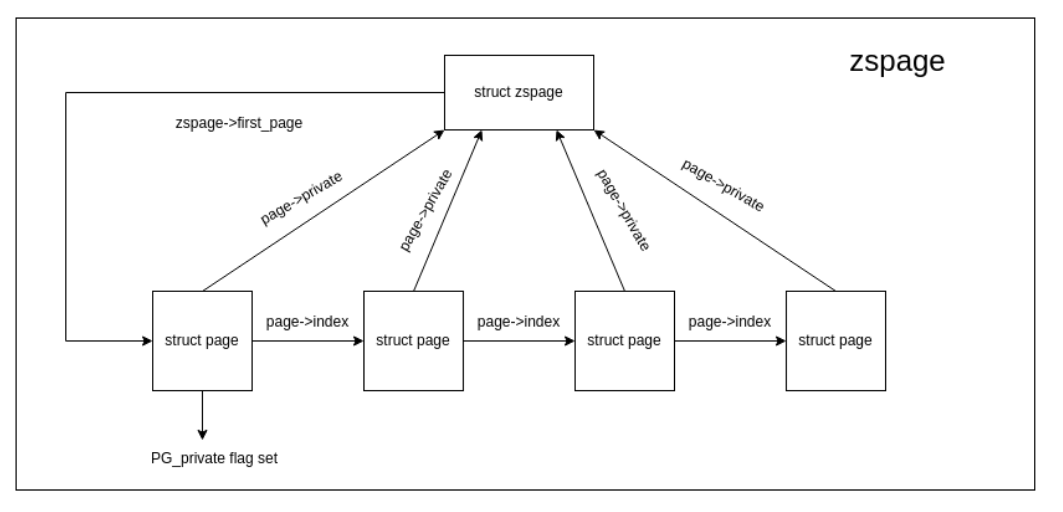
\includegraphics[width=0.95\textwidth]{img/zspage.png}
	\caption{Схематическое описание структуры данных zspage}
	\label{fig:zspage}
\end{figure}

Структуры \texttt{struct page} связаны друг с другом при помощи поля \texttt{index}, которое является указателем на начало каждой последующей страницы списка. Для вычисления, к какой именно структуре zspage страница относится, используется поле \texttt{private}, являющееся указателем на соответствующую структуру \texttt{struct zspage}. У первой странице в списке установлен флаг \texttt{PG\_private}, а так же структура \texttt{struct zspage} имеет указатель на эту страницу. Максимум в списке может быть 4 страницы, минимум -- одна.

На рисунке \ref{fig:zspage_mem} представлено расположение выделяемых объектов в памяти.

\begin{figure}[h]
	\centering
	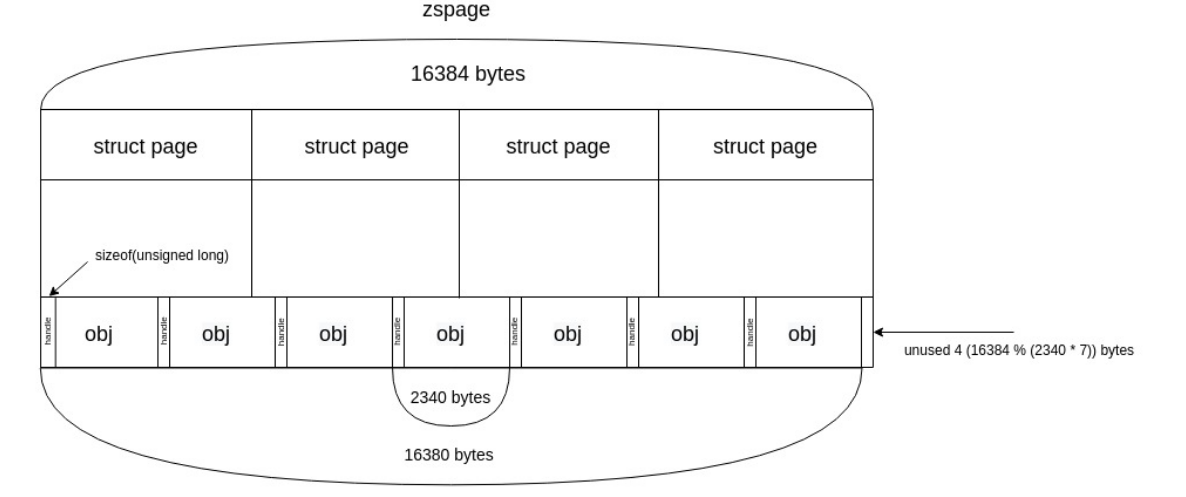
\includegraphics[width=\textwidth]{img/zspage_mem.png}
	\caption{Расположение объектов, хранящихся в zspage, в памяти}
	\label{fig:zspage_mem}
\end{figure}

Объекты (обозначены именем \texttt{obj}), находятся в памяти друг за другом. Перед каждым находится его дескриптор, размер которого соответствует\\ \texttt{sizeof(unsigned long)}. Это некоторое целое, безналичное число, которое кодирует положение данного объекта в памяти. В случае, если объект не выделен, дескриптор указывает на следующий свободный объект, тем самым формируя список свободных объектов внутри zspage. 

На рисунке \ref{fig:handle} представлено описание дескриптора, описывающего запрашиваемые у аллокатора объекты. 

\begin{figure}[h]
	\centering
	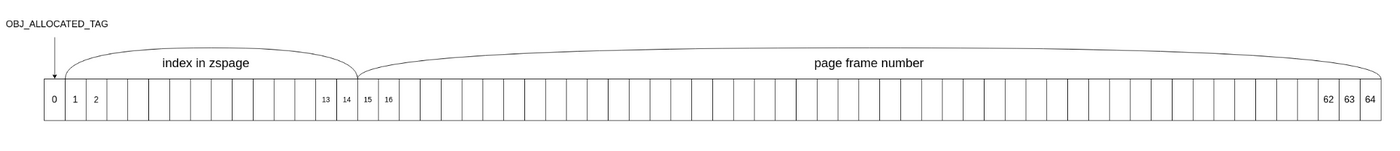
\includegraphics[width=\textwidth]{img/handle.png}
	\caption{Дескриптор объекта}
	\label{fig:handle}
\end{figure}

Дескриптор представляется из себя целое число, состоящее из \\ \texttt{sizeof(unsigned long)} байт. Для простоты изложения, его размер указан в качестве 8 байт (64 бита). 

Первый бит является тегом, позволяющим определить, свободен ли объект. Если первый бит установлен в 0, это значит, что область памяти, находящаяся за дескриптором, не используется. В таком случае, оставшиеся 63 бита являются указателем на следующий свободный участок памяти. В обратном случае (то есть объект уже кем-то используется) биты с 1 по 14 описывают индекс объекта внутри zspage. Оставшиеся биты являются порядковым номером страницы \texttt{struct page} в глобальном массиве \texttt{mem\_map}, который был описан ранее. При выделении объекта, функция \texttt{zs\_malloc} возвращает данный дескриптор.

Страницы zspage связаны друг с другом с помощью связанного списка. Для каждого размера объекта, в системе существует 4 связанных списка, хранящие страницы zspage:

\begin{itemize}
	\item \texttt{ZS\_EMPTY} -- список, хранящий страницы zspage в которых все объекты свободны;
	\item \texttt{ZS\_FULL} -- список zspage, в которых все объекты заняты;
	\item \texttt{ZS\_ALMOST\_EMPTY} -- список zspage, в которых количество занятых объектов не превышает $\frac{3 * obj}{4}$, где \texttt{obj} -- общее количество объектов в странице;
	\item \texttt{ZS\_ALMOST\_FULL} -- список zspage, не попавшими ни в один из вышеперечисленных списков.
\end{itemize}

На рисунке \ref{fig:fullness_group} представлено взаимодействие списков \texttt{ZS\_EMPTY}, \texttt{ZS\_FULL}, \texttt{ZS\_ALMOST\_EMPTY}, \texttt{ZS\_ALMOST\_FULL} и страниц zspage. 

\begin{figure}[h]
	\centering
	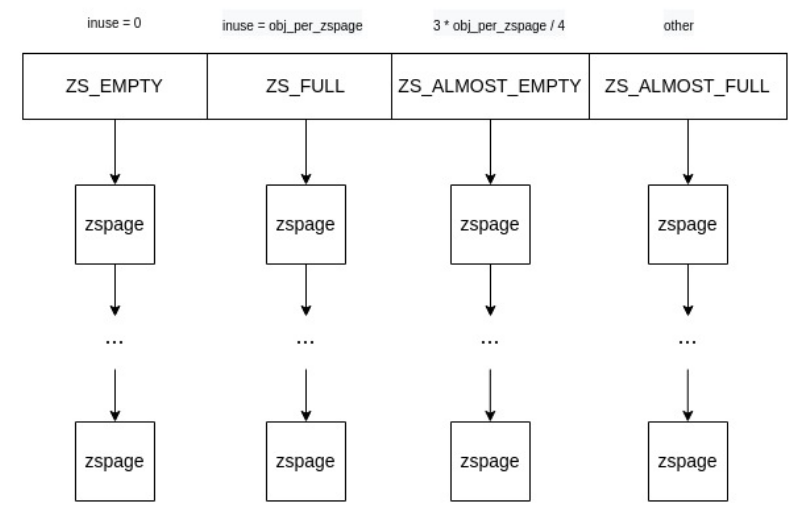
\includegraphics[width=\textwidth]{img/fullness_group.png}
	\caption{Взаимодействие zspage}
	\label{fig:fullness_group}
\end{figure}

Для эффективного размещения объектов разного размера в памяти, используется структуры данных называемая size class и zspool, в исходном коде описываемые соответственно структурами \texttt{struct size\_class} и {struct zs\_pool} (см. листинги \ref{code:size_class} -- \ref{code:zs_pool}).

\begin{code}
	\captionof{listing}{Структура \texttt{struct size\_class}}
	\label{code:size_class}
	\inputminted
	[
	frame=single,
	framerule=0.5pt,
	framesep=20pt,
	fontsize=\small,
	tabsize=4,
	linenos,
	numbersep=5pt,
	xleftmargin=10pt,
	]
	{text}
	{code/size_class.c}
\end{code}

Структура данных size\_class предназначена для хранения всех объектов размером \texttt{size}. Данная структура данных хранит в себе указатели на  четыре списка, описанных ранее, которые в свою очередь указывают на страницы zspage. Поле \texttt{objs\_per\_zspage} хранит в себе количество объектов, размещаемых в страницах zspage для данного size class, а в поле \texttt{page\_per\_zspage} хранится количество страниц памяти, используемых внутри zspage.

\begin{code}
	\captionof{listing}{Структура \texttt{struct zs\_pool}}
	\label{code:zs_pool}
	\inputminted
	[
	frame=single,
	framerule=0.5pt,
	framesep=20pt,
	fontsize=\small,
	tabsize=4,
	linenos,
	numbersep=5pt,
	xleftmargin=10pt,
	]
	{text}
	{code/zs_pool.c}
\end{code}

zspool -- самая <<верхняя>> структура данных, используемая в алгоритме работы аллокатора zsmalloc. Данная структура хранит в себе массив типа \\ \texttt{size\_class}, таким образом, каждому пулу принадлежит \texttt{ZS\_SIZE\_CLASSES} соответствующих структур. Суть заключается в том, что каждый size\_class отличается от предыдущего размером объектов, которые он хранит. Таким образом, самый size\_class хранит объекты размером \texttt{PAGE\_SIZE}, второй объекты размером \texttt{PAGE\_SIZE - C}, третий \texttt{PAGE\_SIZE - 2 * C} и так далее. На данный момент, $C = 8$, что позволяет создать до 255 size class, при размере страницы 4 Кб. При запросе у аллокатора участка памяти размером $n$ байт, $n$ будет округлено до ближайшего размера size class. Несмотря на то, что размер будет округлен, благодаря большому количеству size class, количество на самом деле неиспользуемых байт будет минимально возможным.  Такой подход позволяет максимально эффективно распределять и управлять участками памяти.

На рисунке \ref{fig:zsmalloc_full} представлено взаимодействие всех описанных в этом разделе структур данных.

\begin{figure}[h]
	\centering
	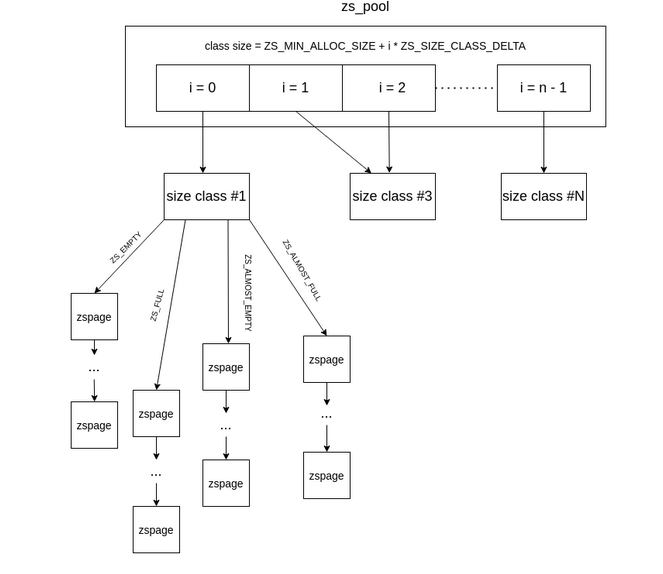
\includegraphics[width=\textwidth]{img/zsmalloc_full.png}
	\caption{Взаимодействие структур данных аллокатора zsmalloc}
	\label{fig:zsmalloc_full}
\end{figure}

Недостатком аллокатора zsmalloc является тот факт, что он предназначен для работы лишь с объектами, размер которых не превышает \texttt{PAGE\_SIZE} байт.

\subsection{Управление несмежными областями памяти}

Области в памяти предпочтительно отображать в последовательности физически смежных страниц памяти, обеспечивая эффективное использование кэша и уменьшая среднее время доступа к памяти. Если запросы на области памяти происходят нечасто, или для решаемой задачи не имеет значение физическая смежность страниц, можно использовать схему, основанную на физически несмежных страницах, обращение к которым происходит смежные линейные адреса. Такой подход позволяет избегать внешней фрагментации, но, при этом, заставляет менять таблицу страниц.

В ядре Linux есть специальный участок памяти, зарезервированный для аллокаций такого типа. На рисунке \ref{fig:vmalloc_area} представлен такой участок. 

\begin{itemize}
	\item интервал \texttt{PAGE\_OFFSET} -- \texttt{high\_memory} -- включает в себя отображение первых 896 Мбайт оперативной памяти
	\item конец области, то есть интервал, начинающийся с \texttt{FIXADDR\_START}, содержит фиксированно отображенные линейные адреса;
	\item в интервале \texttt{PKMAP\_BASE} -- \texttt{FIXADDR\_START} находятся адреса, используемые для постоянного отображения ядром страниц памяти;
	\item остальные адреса используются под смежные области памяти. Интервалы 8 Мб между \texttt{high\_memory} и \texttt{VMALLOC\_START} необходим для обеспечения безопасности и отлавливания обращения памяти по некорректным адресам. По той же самой причине между несмежными областями памяти есть дополнительные интервалы разделом 4 Кб.
\end{itemize}

Таким образом, для выделения несмежных областей памяти, используются адреса расположенные между \texttt{VMALLOC\_START} и \texttt{VMALLOC\_END}.

\begin{figure}[h]
	\centering
	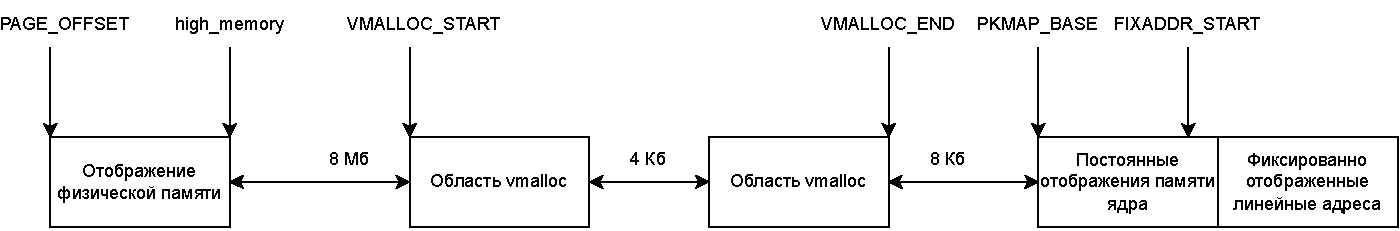
\includegraphics[width=\textwidth]{img/memory-layout.pdf}
	\caption{Интервал линейный адресов, начинающийся с \texttt{PAGE\_OFFSET}}
	\label{fig:vmalloc_area}
\end{figure}

Для описания каждой несмежной области памяти в ядре Linux используется структура \texttt{struct vm\_struct}, описание которой представлено в листинге \ref{code:vm_struct}. Рассматриваемые дескрипторы объединены в простой односвязный список с помощью поля \texttt{next}.

\begin{code}
	\captionof{listing}{Структура \texttt{struct vm\_struct}}
	\label{code:vm_struct}
	\inputminted
	[
	frame=single,
	framerule=0.5pt,
	framesep=20pt,
	fontsize=\small,
	tabsize=4,
	linenos,
	numbersep=5pt,
	xleftmargin=10pt,
	]
	{text}
	{code/vm_struct.c}
\end{code}

Ниже представлено подробное описание полей:

\begin{itemize}
	\item \texttt{addr} -- линейный адрес первой ячейки памяти;
	\item \texttt{size} -- размер области + 4 Кб;
	\item \texttt{flags} -- флаги, описывающие область памяти;
	\item \texttt{pages} -- указатель на массив из \texttt{nr\_pages} указателей на дескрипторы страниц;
	\item \texttt{nr\_pages} -- количество страниц, расположенных в области;
\end{itemize}

Для выделения несмежной области памяти в ядре Linux используются API, представленной в листинге \ref{code:vm_api}.

\begin{code}
	\captionof{listing}{API для работы с несмежными областями памяти}
	\label{code:vm_api}
	\inputminted
	[
	frame=single,
	framerule=0.5pt,
	framesep=20pt,
	fontsize=\small,
	tabsize=4,
	linenos,
	numbersep=5pt,
	xleftmargin=10pt,
	]
	{text}
	{code/vm_api.c}
\end{code}

Функция \texttt{vmalloc} используется для выделения несмежной области памяти размером \texttt{size}, а функция \texttt{vfree} соответственно для освобождения такой области памяти. При запросе такой области памяти, функция сначала находит подходящую область памяти, которая описывается структурой \texttt{struct vm\_struct} и меняет таблицы страниц таким образом, чтобы страницы, на которые указывает эта структура отображались в соответствующие линейные адреса. 

Функция \texttt{vmap} и \texttt{vunmap} работает аналогично, за исключение того, что физические страницы, которые нужно отобразить в соответствующие линейные адреса передаются в качестве параметра.

Данный способ выделения памяти является затратным, так как пользуется изменением страниц, что чревато увеличением времени доступа памяти и отзывчивости всей системы в целом.

\subsection{Классификация методов распределения памяти}

Для классификации рассмотренных ранее методов были выделены следующие критерии:

\begin{itemize}
	\item К1 -- использование физически смежных адресов памяти
	\item К2 -- произвольный размер запрашиваемой области памяти;
	\item К3 -- максимально возможная утилизация памяти;
	\item К4 -- успешная аллокация в условиях нехватки памяти;
\end{itemize}

Результаты классификации рассматриваемых методов описаны в таблице \ref{tbl:comparsion}.

\begin{table}[h]
	\small
	\caption{Классификация методов распределения памяти в ядре Linux}
	\label{tbl:comparsion}
	\begin{center}
	\begin{tabular}{|l|l|l|l|l|}
		\hline
		Метод & К1 & К2 & К3 & К4 \\ \hline
		Buddy аллокатор  & + & - & + & +\\ \hline
		Slab аллокатор & + & + / - & - & -\\ \hline
		Пулы памяти & + & - & + & + \\ \hline
		zsmalloc & + & - & + + & + \\ \hline
		vmalloc & - & + & + & - \\ \hline
	\end{tabular}
\end{center}
\end{table}

В случае Slab аллокатора, при использовании функции \texttt{kmalloc}, то есть при обращении к общему кэшу с геометрически распределенными размерами, запрос области памяти возможен, а в случае использования функции \\ \texttt{kmem\_cache\_alloc} -- нет.

Таким образом, нельзя сделать вывод о универсальности какого-либо метода. Каждый метод необходимо использовать для решения конкретной задачи в конкретной ситуации.

\pagebreak
